\documentclass[mathserif, 12pt, t]{beamer}

\let\Tiny=\tiny


\usepackage{graphicx}
\usepackage{float}
% \usepackage{enumitem}
\usepackage{natbib}
\usepackage{amsmath}
\usepackage{bm}
\usepackage{dsfont}
\geometry{vmargin=0.5in}


%%% Do not overwrite a defined color (#1) if already defined,
%%% otherwise set the color to rgb(#2)
\makeatletter
\newcommand{\colorprovide}[2]{%
    \@ifundefinedcolor{#1}{\definecolor{#1}{rgb}{#2}}{}}
\makeatother

%colors
\colorprovide{colorheader}{0.00, 0.40, 1.00}
\colorprovide{colortitle}{0.00, 0.24, 0.60}
\colorprovide{colorfootertext}{0.00, 0.45, 0.80}
\colorprovide{colorfooter}{0.00, 0.00, 0.00}

\setbeamercolor{local structure}{fg=colortitle}

\setbeamercolor{footlinecolor}{bg=colorfooter,fg=colorfootertext}

\beamertemplatenavigationsymbolsempty
\setbeamertemplate{footline}{%
    \hbox{%
    \vspace{0.5in}%
    \begin{beamercolorbox}[ht=2mm, rightskip=.5cm]{footlinecolor}%
    \hfill\insertframenumber/\inserttotalframenumber
    \end{beamercolorbox}}}


%\bibpunct{(}{)}{;}{a}{}{,}

%commands
\newcommand{\citei}[1]{\phantom{\cite{#1}}\vspace{-14pt}}

\newcommand{\ind}{\mathds{1}}
\newcommand{\m}[1]{\mathbf{\bm{#1}}}
\newcommand{\R}{I\hspace{-4.4pt}R}

\renewcommand{\frametitle}[1]{\vspace{0.14cm}\hspace{-0.70cm}\textcolor{colortitle}{%
    \textbf{\large{#1}}}\vspace{0.15cm}\newline}


\newcommand{\startappendix}{%
    \setbeamertemplate{footline}{%
        \hbox{%
        \vspace{0.5in}%
        \begin{beamercolorbox}[ht=2mm, rightskip=.5cm]{footlinecolor}%
        \hfill A\the\value{framenumberappendix}\phantom{/\inserttotalframenumber}
        \end{beamercolorbox}}}
    \newcounter{framenumberappendix}
    \setcounter{framenumberappendix}{0}
    }


%slide colors
\pagecolor{colorheader!60}

% title page slide
\renewcommand{\titlepage}[4]{%
    {
    \setbeamertemplate{footline}{%
        \hbox{%
        \vspace{0.5in}%
        \begin{beamercolorbox}[ht=2mm, rightskip=.5cm]{footlinecolor}%
        \phantom{/}
        \end{beamercolorbox}}}
    \begin{frame}
    %\begin{center}
    \ \\ [-0.5in]
    \vfill
    \bigskip
    \bigskip
    \bigskip
    \bigskip
    \bigskip


    %\end{center}
    \begin{large}
    #1
    \end{large}
    %\begin{center}
    \vfill

    #2
    \vfill

    #3
    \smallskip

    #4

    \bigskip
    \bigskip
    \vfill
    \ \\ [-0.5in]
    %\end{center}
    \end{frame}
    }
    \addtocounter{framenumber}{-1}
    }


\newcommand{\bc}[1]{\textcolor{blue}{\mathbf{#1}}}

\begin{document}

%\titlepage{Dirichlet process mixture model applied to Hopkinson-bar experiments}{Mickey Warner}{7 December 2015}{AMS 241}
\titlepage{Dirichlet process mixture model on Hopkinson-bar experiments}{Mickey Warner}{7 December 2015}{AMS 241}

%\begin{frame}
%\frametitle{Goal}
%
%Use a Dirichlet process mixture (DPM) model for multivariate data with a non-conjugate baseline distribution.
%
%\end{frame}


\begin{frame}{Data: simulated}

\begin{minipage}{0.60\textwidth}
Generated $n=100$ curves, each of length $k_i$,
\[ \m{y}_i = \beta_{i0}\m{1}_{k_i} + \beta_{i1}\m{x}_i + \beta_{i2}\m{x}_i^2 + \m{\epsilon}_i \]
where

\begin{itemize}[label=$\cdot$]
\item $\m{\epsilon}_i~ \overset{iid}\sim N(0, 0.05^2\m{I}_{k_i})$
\item $\beta_{i0} \overset{iid}\sim N(3, 0.3^2)$
\item $\beta_{i1} \overset{iid}\sim N(1.5, 0.1^2)$
\item $\beta_{i2} \overset{iid}\sim 0.5\delta_0(\cdot) + 0.5N(-1, 0.1^2)$
\end{itemize}

\end{minipage}
\begin{minipage}{0.35\textwidth}
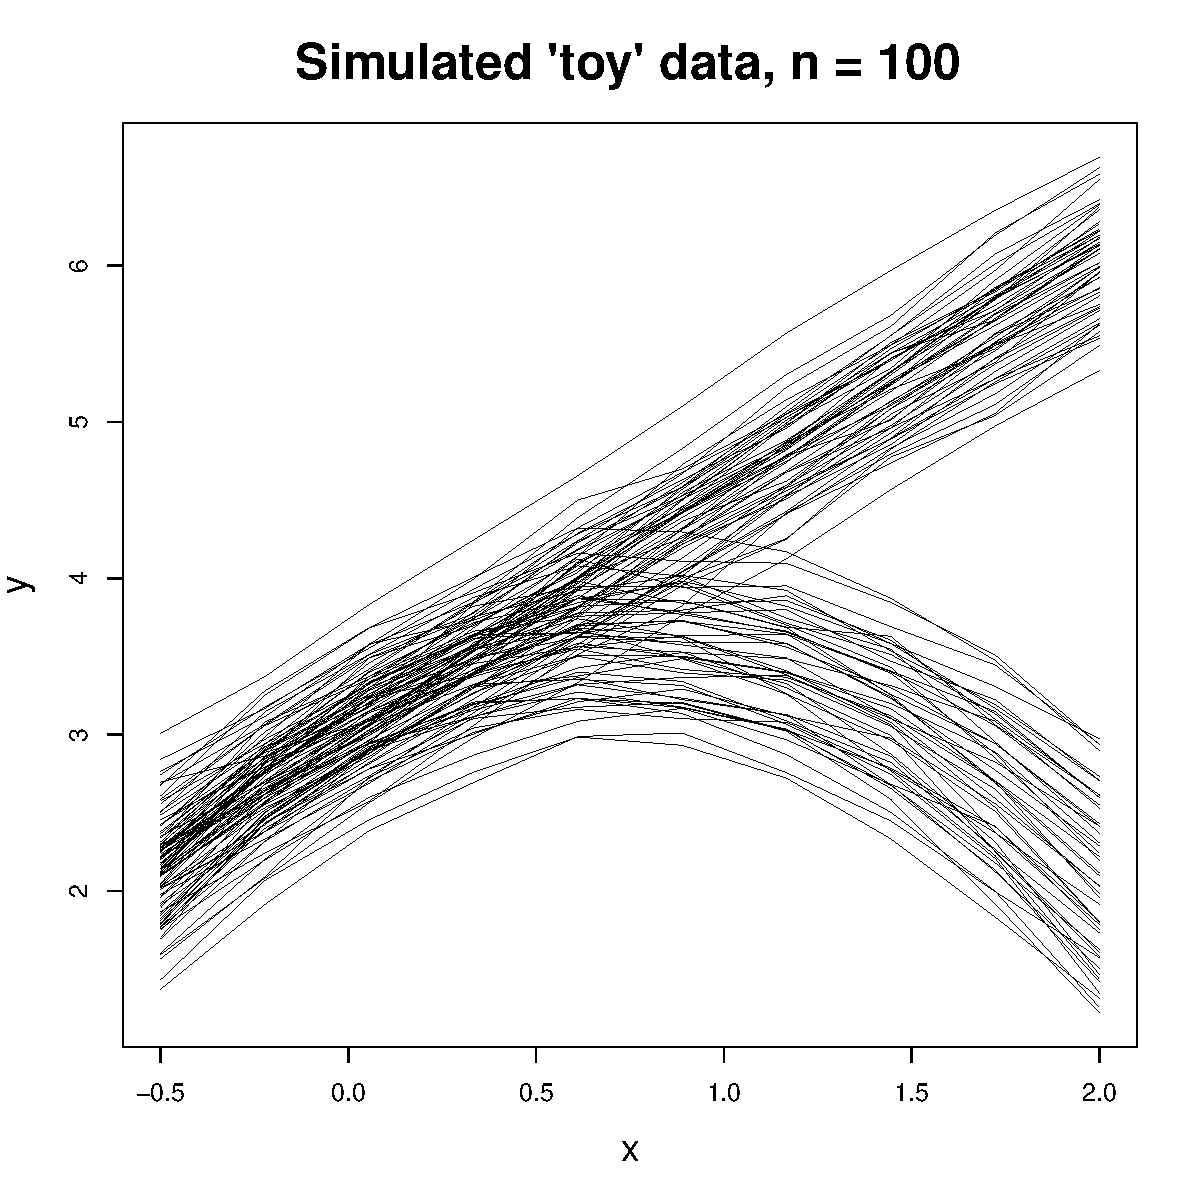
\includegraphics[scale=0.25]{../figs/toy_data.pdf}
\end{minipage}

\end{frame}


\begin{frame}{Data: simulated (continued)}

We use $\m{x}_1=\cdots=\m{x}_n=\m{x}$ that is a vector of $k_i=10$ equally spaced values from $-0.5$ to $2$
\bigskip

Thus we have 100 curves with random intercepts, slopes, and quadratic terms, about half of which are lines and the others are parabolas
\end{frame}

\begin{frame}{Parametric hierarchical model}

The curves $\m{y}_i$ are modeled as a multivariate normal with a quadratic polynomial as the mean:
\begin{align*}
f(\m{y}_i|\m{x}_i,\m{\beta}_i,\tau^2) &= N_{k_i}(\m{y}_i|p(\m{x}_i, \m{\beta}_i), \tau^2\m{I}_{k_i}),~~~~~&i=1,\ldots,n \\
\m{\beta}_i &\overset{iid}\sim N(\m{\mu}, \m{\Sigma}),~~~~~&i=1,\ldots,n \\
\tau^2 &\sim IG(a_\tau, b_\tau) \\
\m{\mu} &\sim N(\m{m}, \m{S}) \\
\m{\Sigma} &\sim IW(\m{V}, d) 
\end{align*}
where $\m{\beta}_i=(\beta_{i0}, \beta_{i1}, \beta_{i2})^\top$, $p(\m{x}_i,\m{\beta}_i) = \beta_{i0}\m{1}_{k_i} + \beta_{i1}\m{x}_i + \beta_{i2}\m{x}_i^2$, and $a_\tau, b_\tau, \m{m}, \m{S}, \m{V}, d$ are specified.

\end{frame}



\begin{frame}{Dirichlet process mixture (DPM) model}

We mix over the parameters in the mean function to obtain
\begin{align*}
f(\m{y}_i|G,\m{x}_i, \tau^2) &= \int N_{k_i}(\m{y}_i|p(\m{x}_i, \m{\beta}), \tau^2\m{I}_{k_i})dG(\m{\beta}) \\
G|\alpha, G_0 &\sim DP(\alpha, G_0=N_p(\m{\beta}|\m{\mu}, \m{\Sigma}))
\end{align*}
and the priors are specified as in the parametric model. %The two models are equivalent, with the exception of the DPM model having a non-parametric prior on the distribution of $\m{\beta}$

\end{frame}

\begin{frame}{Fitting the models}

The priors all yield conjugate posterior conditionals, so sampling can be done easily with Gibbs
\bigskip

For the DPM, since $p(\cdot)$ is a polynomial and $G_0$ is normal, we can use the Gibbs sampler from Escobar and West.

\end{frame}

\begin{frame}{Simulated data: posterior predictive of a new $\m{\beta}_0$}
Black -- parametric; Blue -- DPM)

\begin{center}
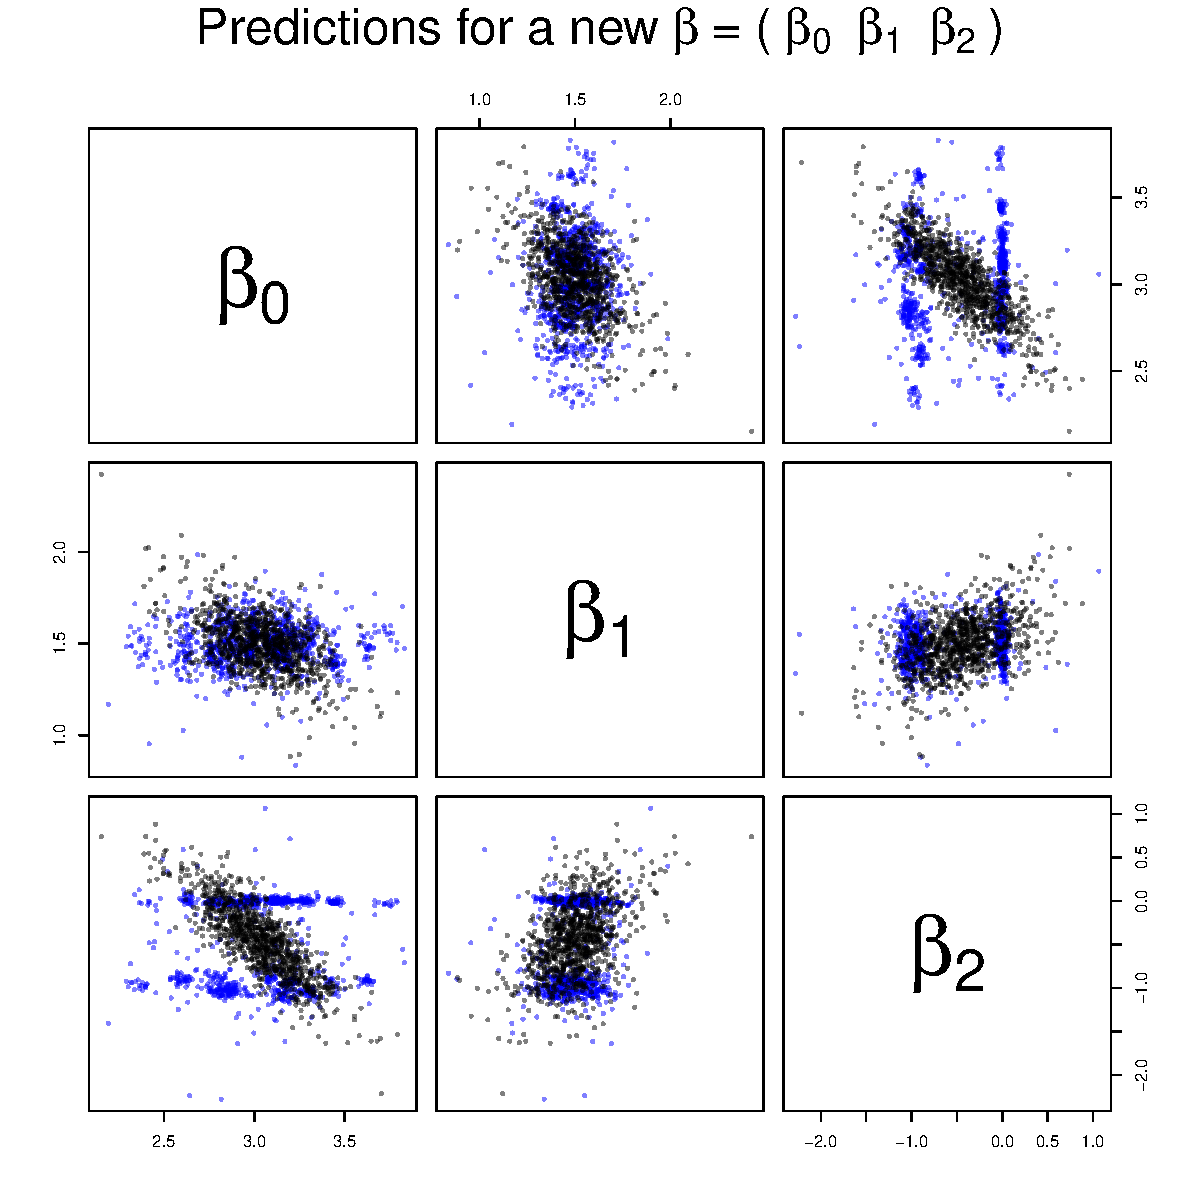
\includegraphics[scale=0.30]{../figs/toy_theta_0.pdf}
\end{center}

\end{frame}

\begin{frame}{Simulated data: posterior predictive of a new $\m{y}_0$}
Based on the posterior predictive for $\m{\beta}_0$

\begin{center}
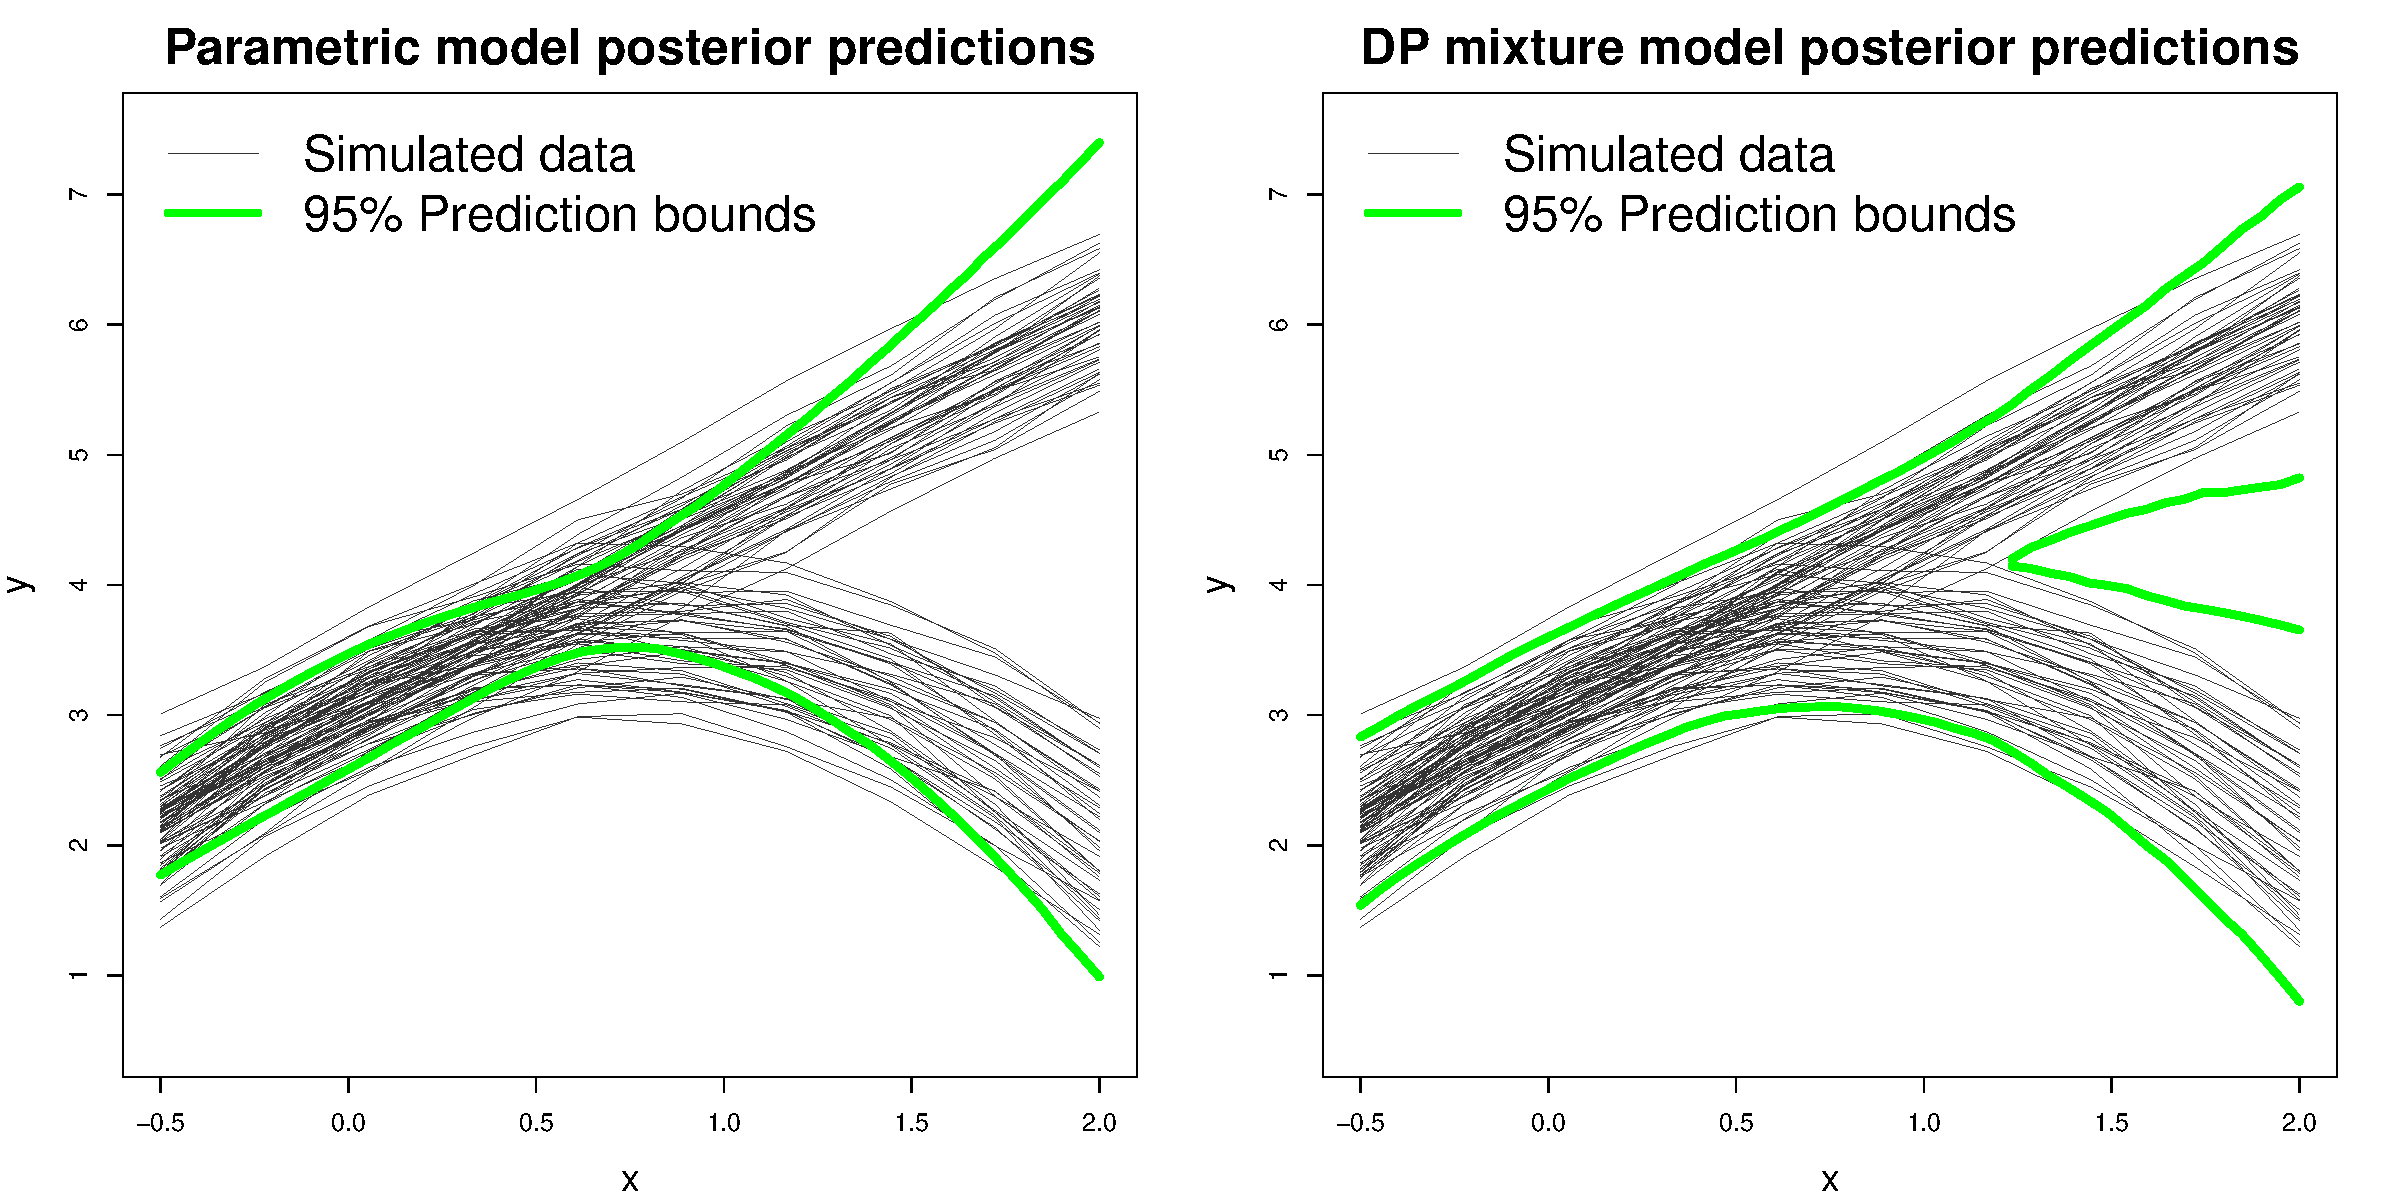
\includegraphics[scale=0.25]{../figs/toy_y_0.pdf}
\end{center}

\end{frame}

\begin{frame}{Hopkinson-bar experiments}

\begin{minipage}{0.50\textwidth}
A small piece of material is compressed or stretched, either slowly or rapidly
\bigskip

The deformation of the material is measured in two ways: stress and strain
\bigskip

Experiments are done at various temperatures and strain rates
\end{minipage}
\begin{minipage}{0.45\textwidth}
\begin{flushright}
\includegraphics[scale=0.50]{../figs/bar_pic.jpg}
\end{flushright}
\end{minipage}

\end{frame}

\begin{frame}{Hopkinson-bar experiments}

\begin{minipage}{0.50\textwidth}
We have curves from $n=10$ experiments
\bigskip

Materials models are typically used to model the data
\bigskip

\end{minipage}
\begin{minipage}{0.45\textwidth}
\begin{flushright}
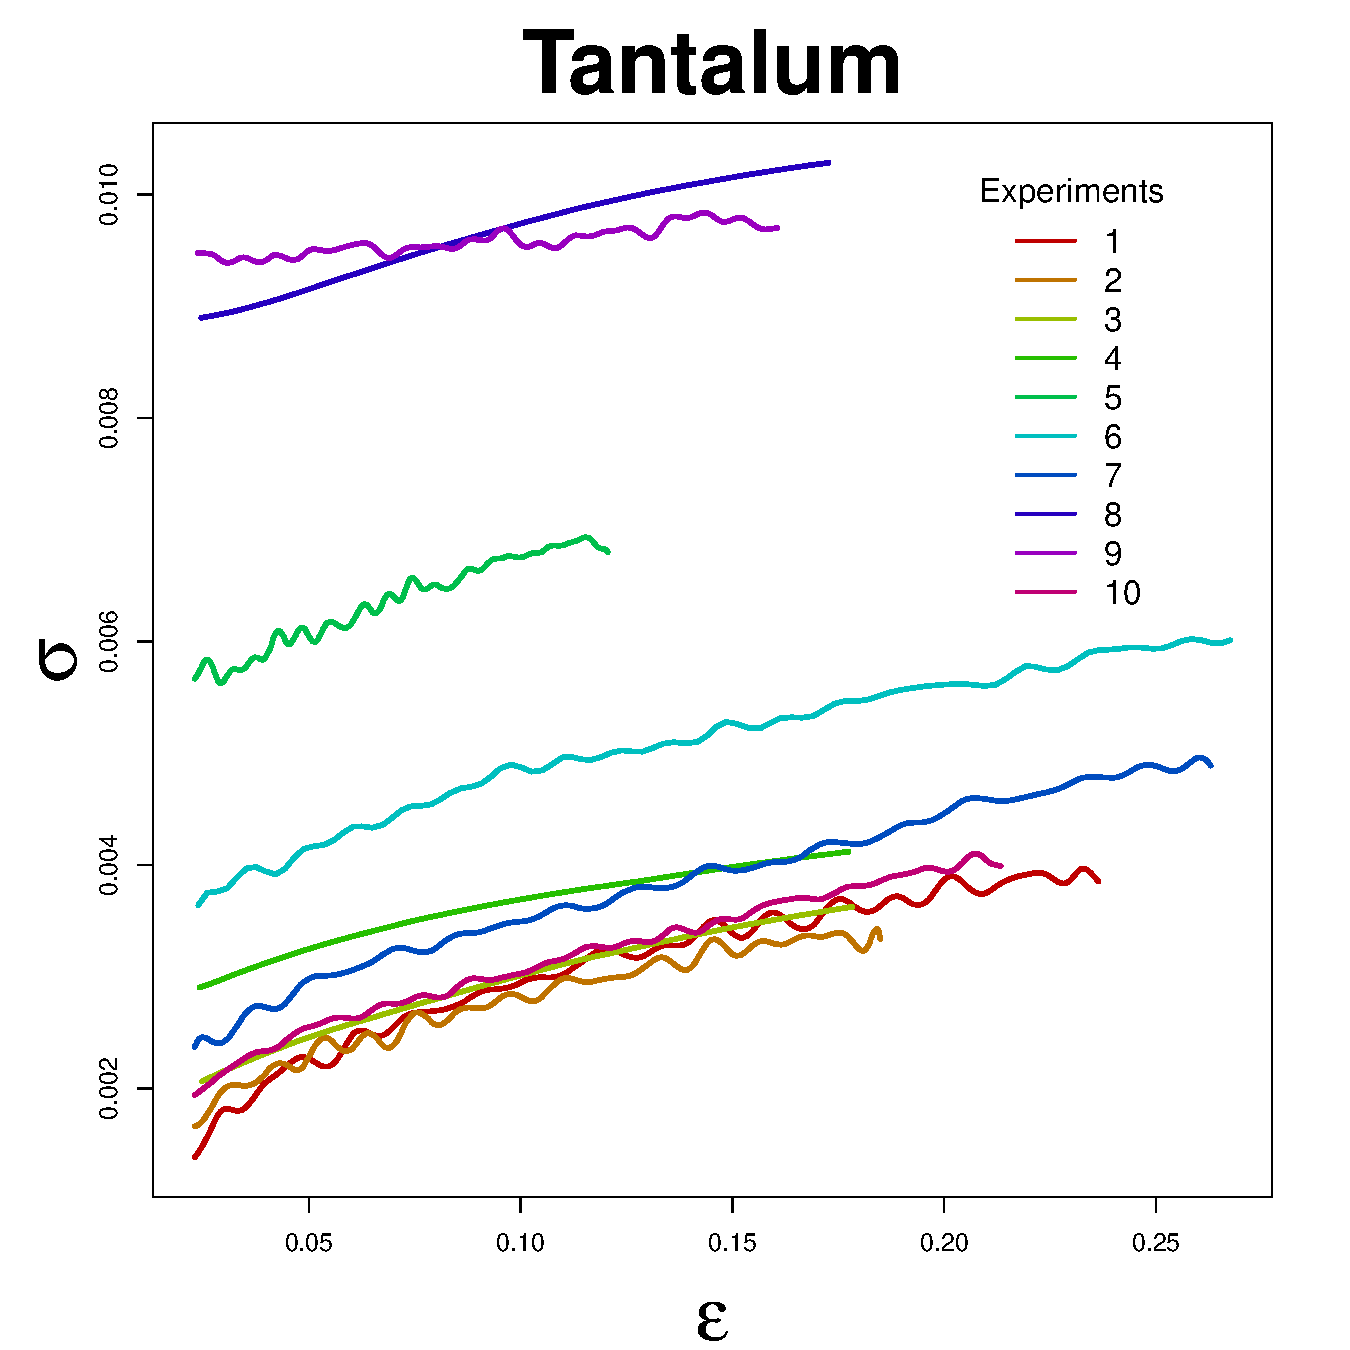
\includegraphics[scale=0.25]{../figs/ta_all_data.pdf}
\end{flushright}
\end{minipage}

\end{frame}

\begin{frame}{Material model}

For $\m{x}=(\m{\epsilon}_p,\dot\epsilon^*,T^*)$ and $\m{\theta}=(A,B,n,C,m)$ the Johnson-Cook model is given by
\[ h(\m{x}, \m{\theta}) = (\bc{A} + \bc{B}\m{\epsilon}_p^{\bc{n}})(1 + \bc{C} \log \dot\epsilon^*)(1 - T^{*\bc{m}}) \]
where $\dot\epsilon^*$ is the experimental strain rate, $T^*$ is the experimental temperature, scaled by melting temperature (in Kelvin), and $\epsilon_p$ is the plastic strain ($x$-axis)
\bigskip

There are other, much better models, but the Johnson-Cook is very simple and is a useful starting point

\end{frame}

\begin{frame}{Statistical models}

Replace $p(\m{x}_i, \m{\beta}_i)$ with the Johnson-Cook model $h(\m{x}_i, \m{\theta}_i)$ for the parametric and semi-parametric models:
\bigskip

Parametric
\[ f(\m{y}_i|\m{x}_i,\m{\theta}_i,\tau^2) = N_{k_i}(\m{y}_i|h(\m{x}_i, \m{\theta}_i), \tau^2\m{I}_{k_i}) \]

DPM
\[ f(\m{y}_i|G,\m{x}_i, \tau^2) = \int N_{k_i}(\m{y}_i|h(\m{x}_i, \m{\theta}), \tau^2\m{I}_{k_i})dG(\m{\theta}) \]

\end{frame}

\begin{frame}{Fitting the models}

Since we no longer have conjugacy with $\m{\theta}$ so we update the latent variables using a Metropolis step (Algorithm 6 from Neal (2000))
\bigskip

All other priors are the same as before and can be updated with Gibbs steps

\end{frame}

\begin{frame}{Posteriors for $\m{\theta}$}
Black -- $\m{\mu}$; colored dots -- means of each $\m{\theta}_i$
\begin{center}
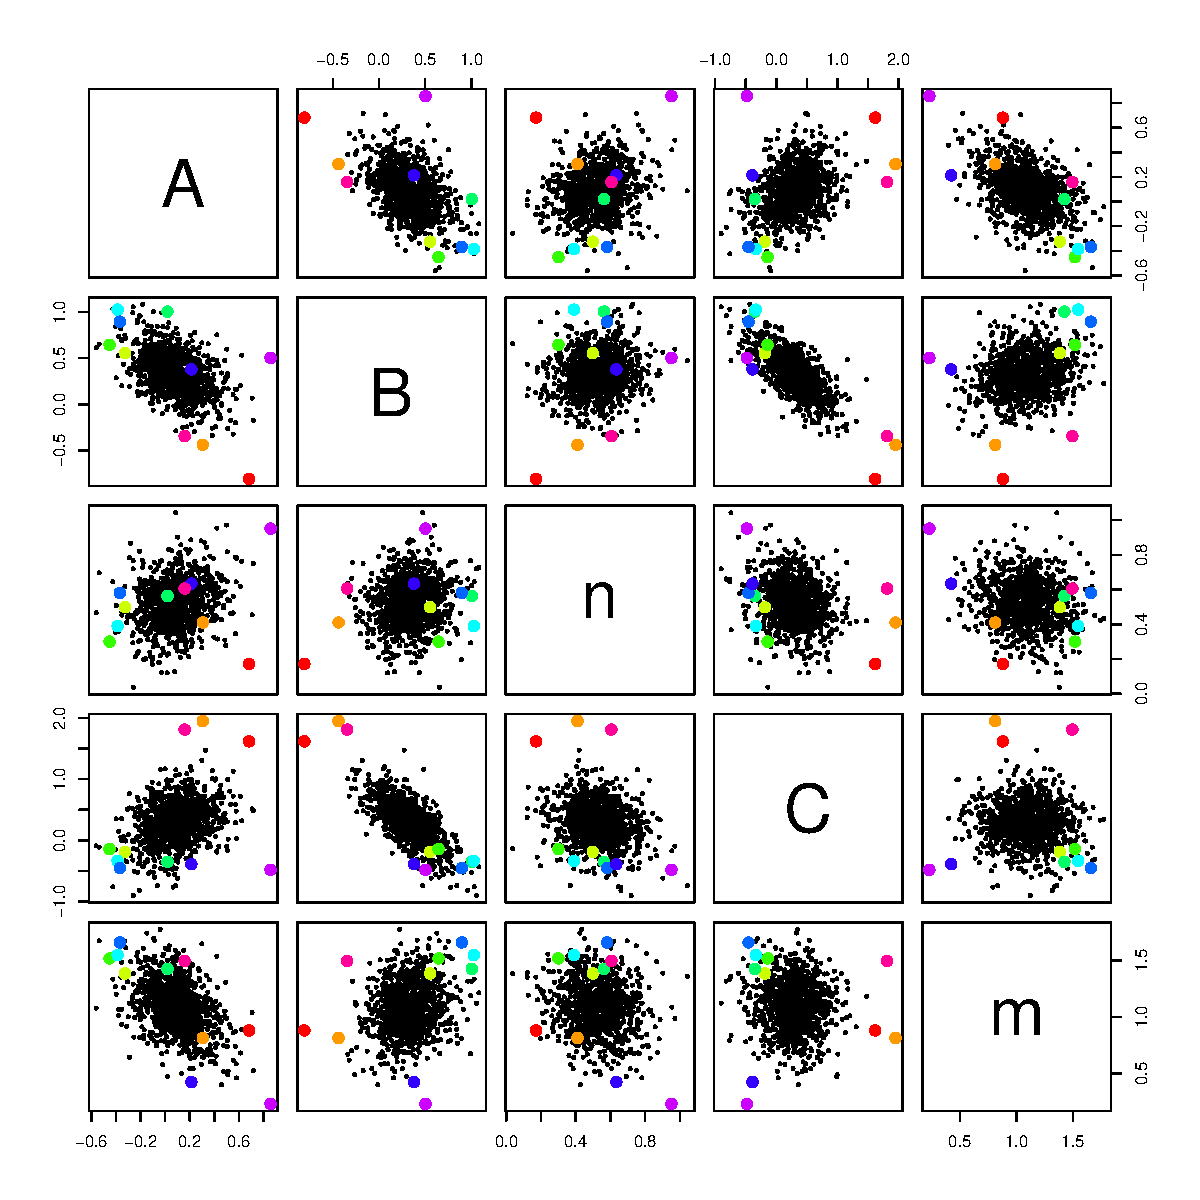
\includegraphics[scale=0.30]{../figs/ms_clusters.pdf}
\end{center}

\end{frame}

\begin{frame}{Predictions (given the random effects)}
\begin{center}
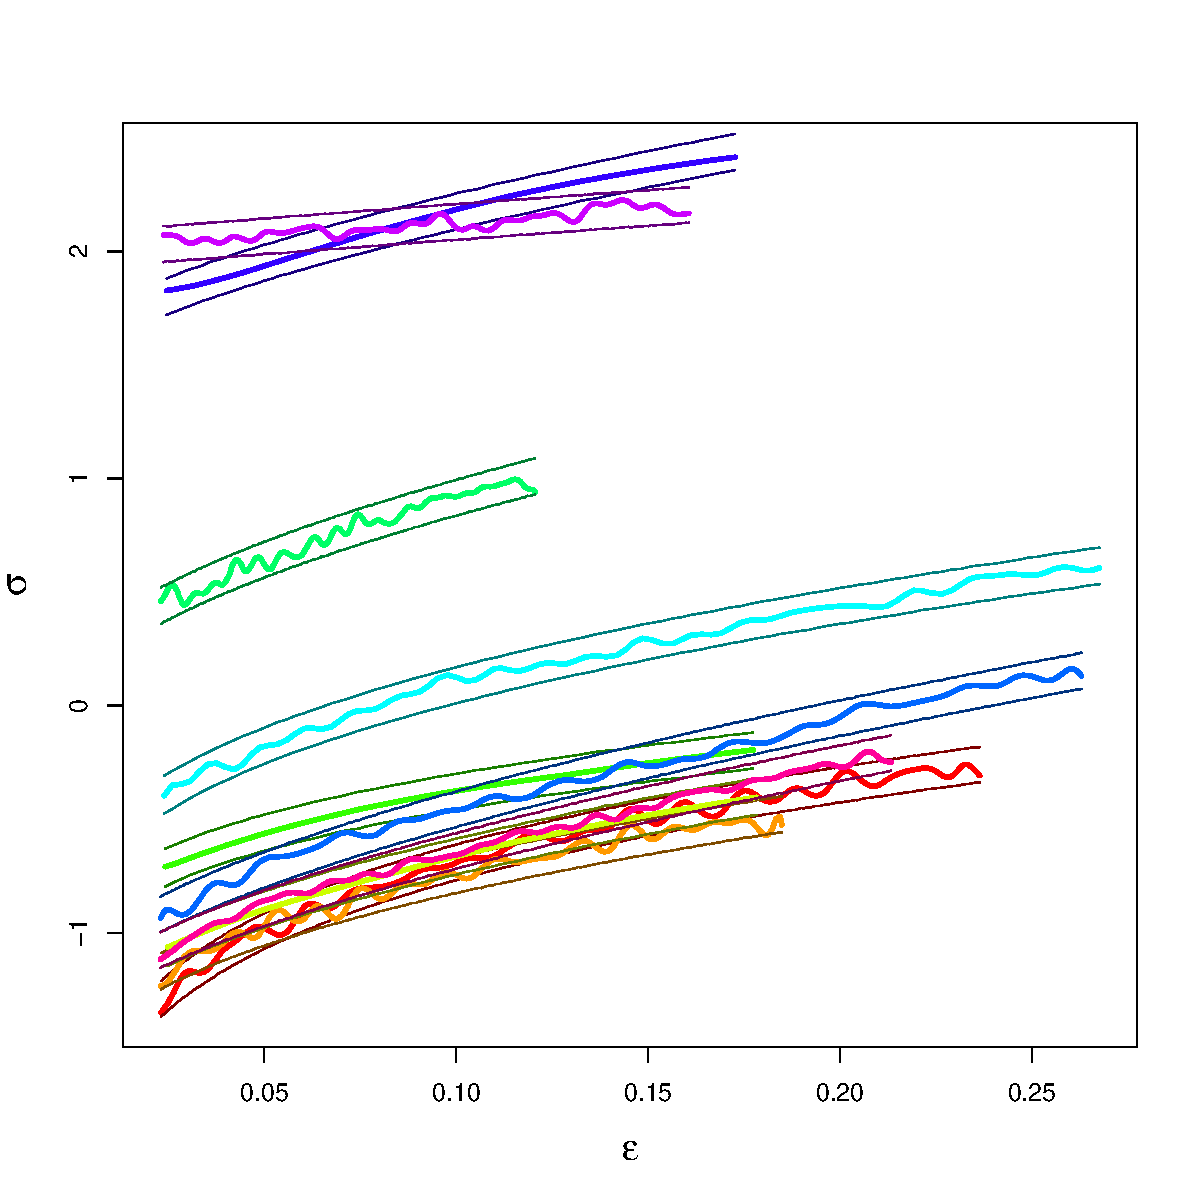
\includegraphics[scale=0.30]{../figs/ms_predsA.pdf}
\end{center}

\end{frame}


\begin{frame}{Conclusions and future work}

Predictions based a new $\m{\theta}_0$ (not shown) were very poor
\bigskip

For covariates $\m{x}^*$ draw a new $\m{\theta}_0$ that are similar to one of the $\m{\theta}_i$'s
\bigskip

Hierarchical DPs? Nested DPs?
\bigskip


\end{frame}

%where $f(\m{x}_i, \m{\theta})$ is a (possibly non-linear) function that maps covariates $\m{x}_i$ and latent variables $\m{\theta}$ to $\R^{k_i}$

%\appendix
%
%\newcounter{finalframe}
%\setcounter{finalframe}{\value{framenumber}}
%
%\begin{frame}{Simulated: posteriors}
%Black -- parametric; Blue -- DPM)
%\begin{center}
%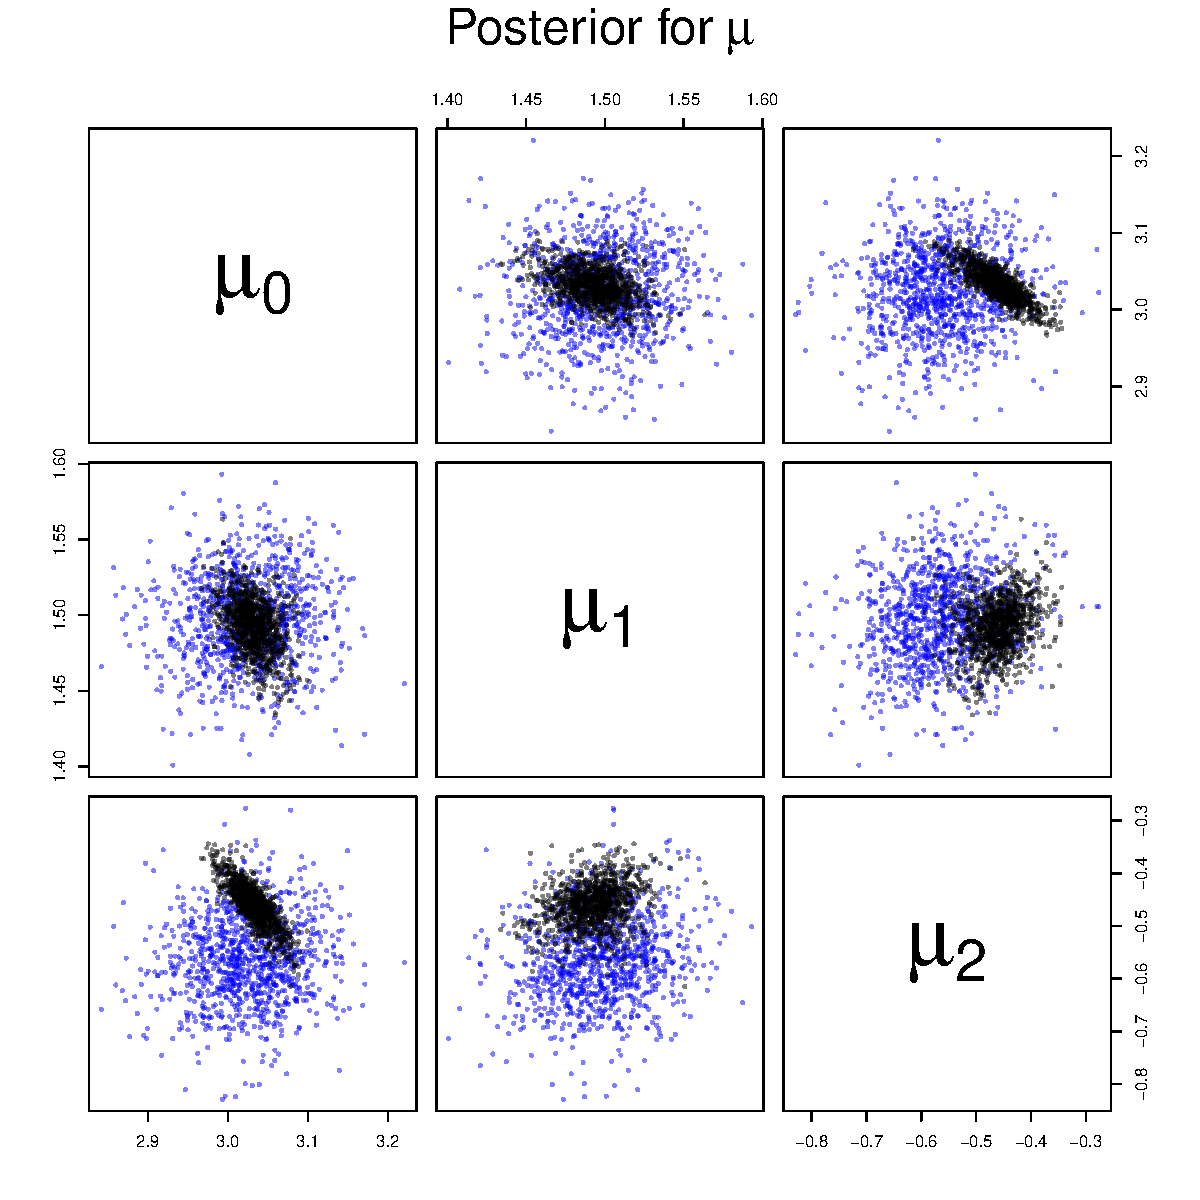
\includegraphics[scale=0.30]{../figs/toy_mu.pdf}
%\end{center}
%\end{frame}
%
%\begin{frame}{Simulated: posteriors}
%Black -- parametric; Blue -- DPM)
%\begin{center}
%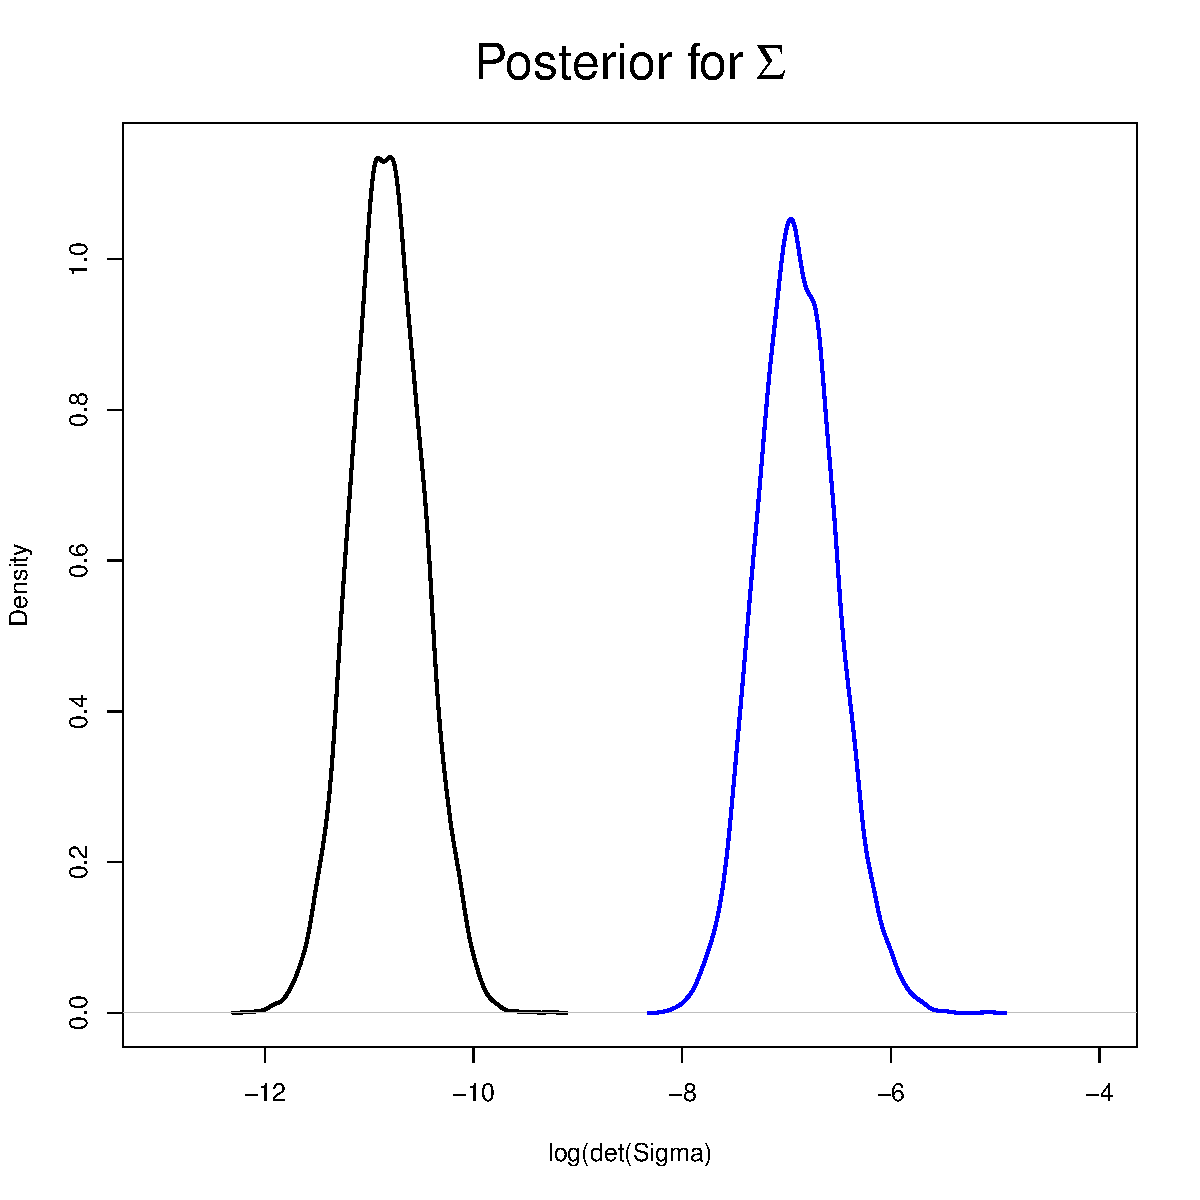
\includegraphics[scale=0.30]{../figs/toy_sigma.pdf}
%\end{center}
%\end{frame}
%
%\begin{frame}{Simulated: posteriors}
%Black -- parametric; Blue -- DPM)
%\begin{center}
%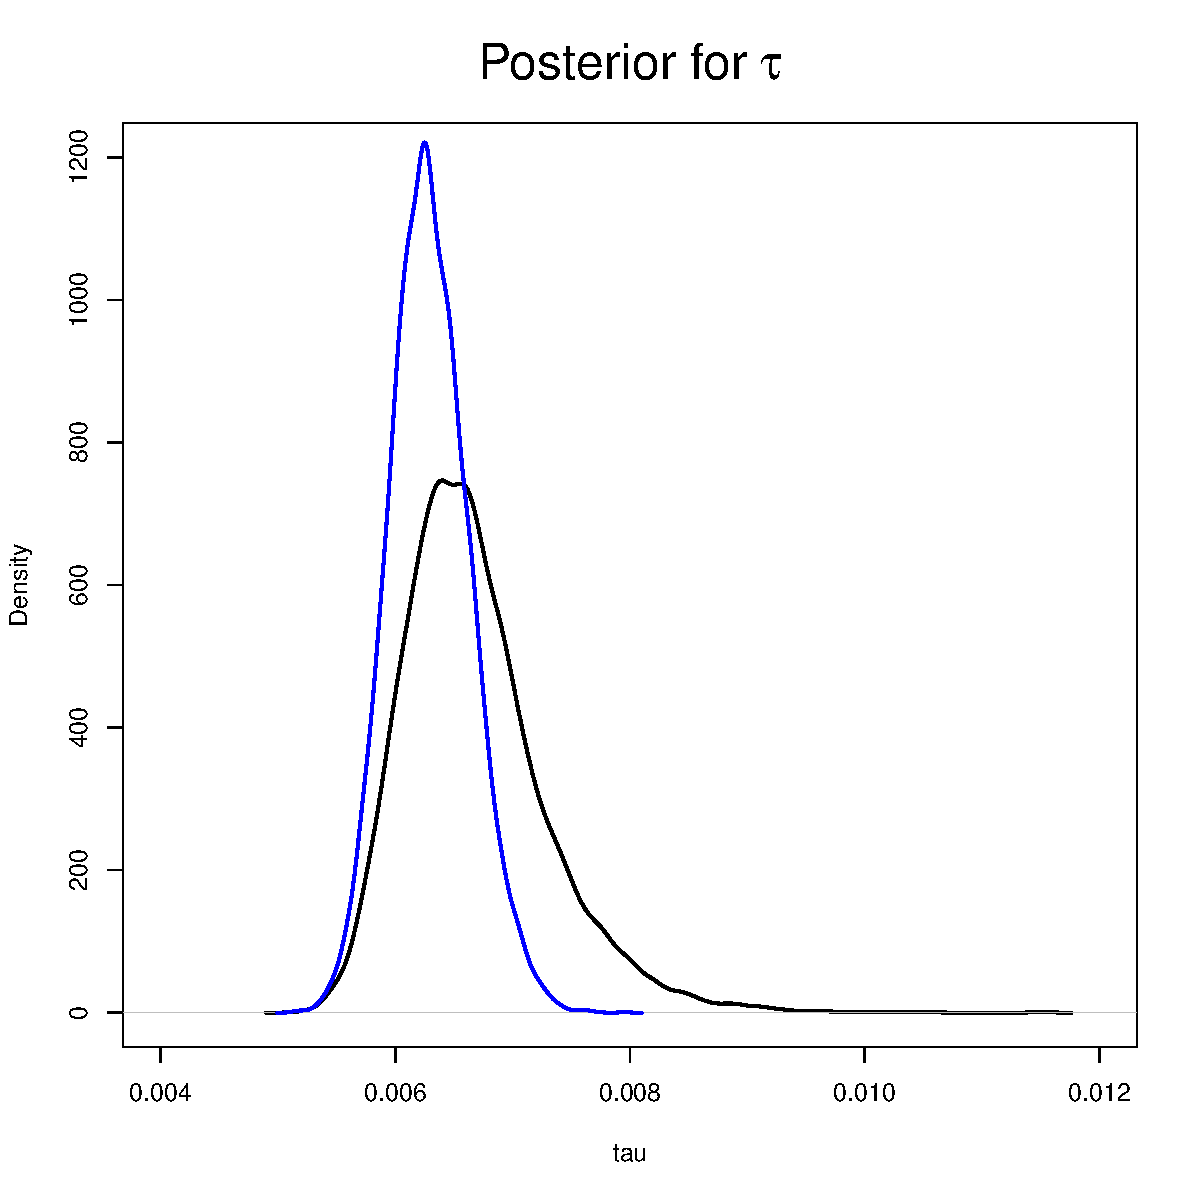
\includegraphics[scale=0.30]{../figs/toy_tau.pdf}
%\end{center}
%\end{frame}
%
%\begin{frame}{Simulated: posteriors (DPM only)}
%\begin{center}
%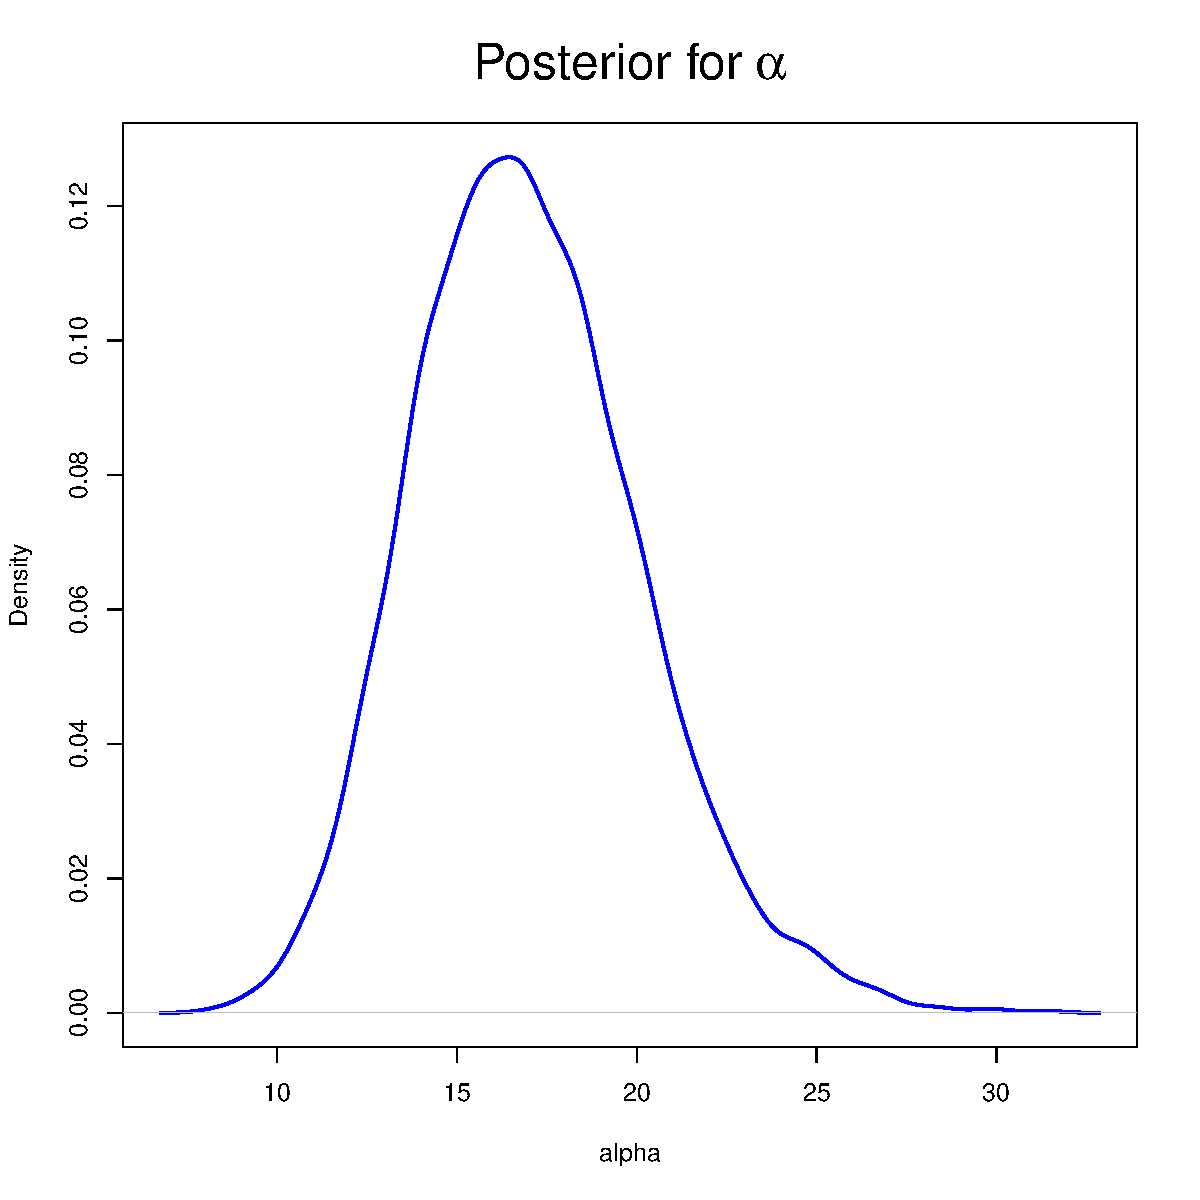
\includegraphics[scale=0.30]{../figs/toy_alpha.pdf}
%\end{center}
%\end{frame}
%
%\begin{frame}{Simulated: log CPO}
%\begin{center}
%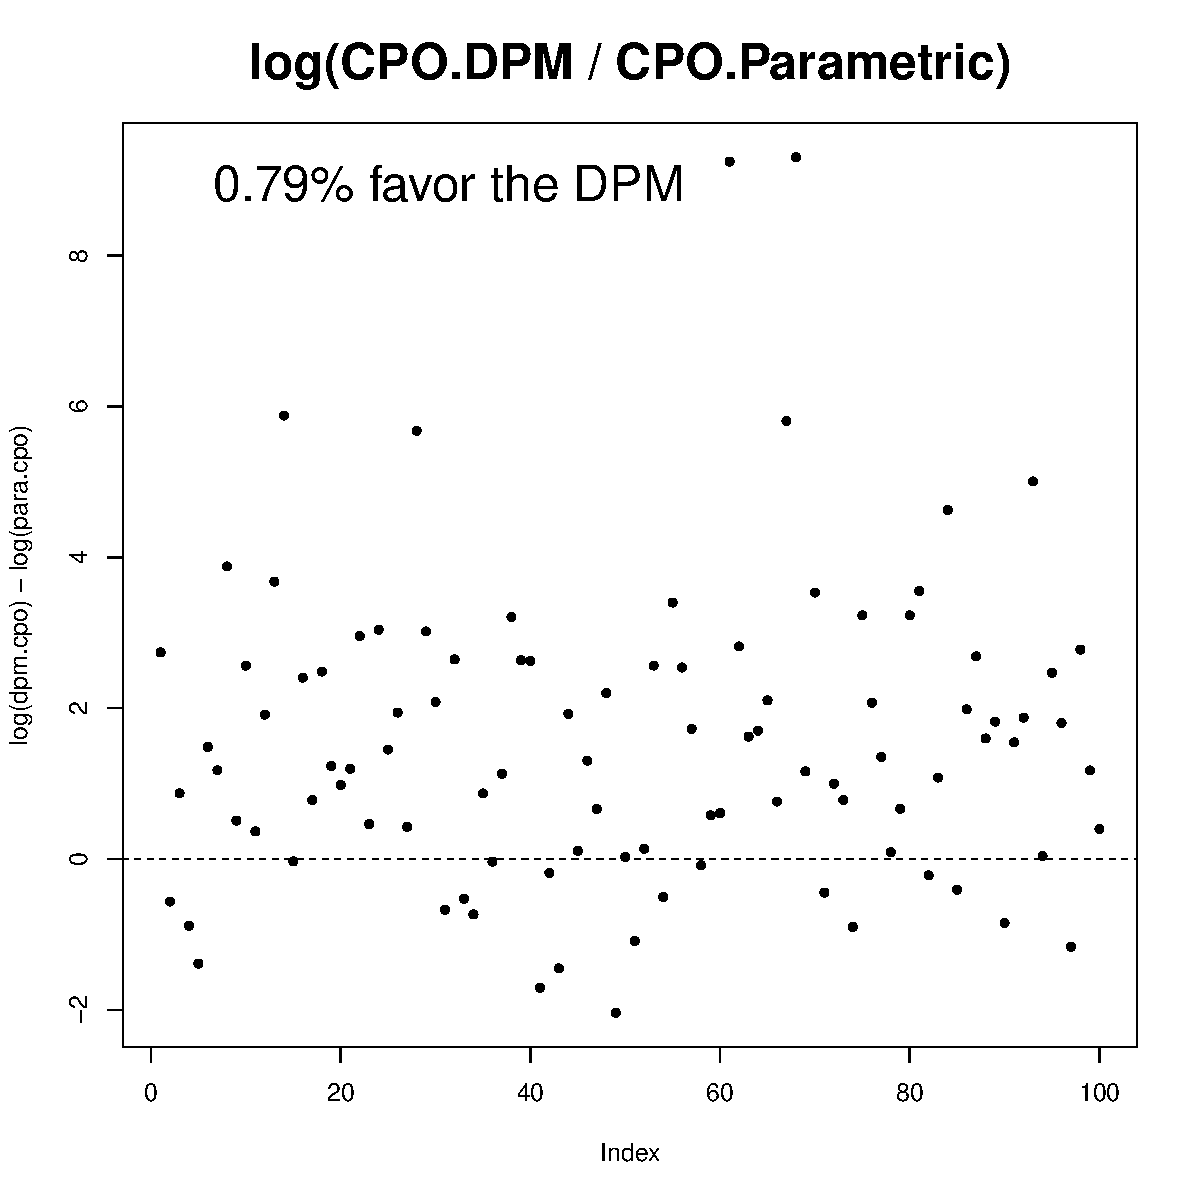
\includegraphics[scale=0.30]{../figs/toy_cpo.pdf}
%\end{center}
%\end{frame}
%
%\setcounter{framenumber}{\value{finalframe}}


\end{document}
